\documentclass{article}

\usepackage[a4paper]{geometry} % document dimensions
\usepackage{amsmath} % multiline equation numbering
\usepackage{amssymb} % e.g. triangleq, checkmark
\usepackage{textcomp,gensymb} % \degree symbol
%\usepackage{bm} % bold symbols numbering
\usepackage{authblk} % author/affiliation block
\usepackage[T1]{fontenc} % support accents via UTF
\usepackage[titletoc,title]{appendix}
\usepackage{booktabs} % e.g. \toprule
\usepackage{pdflscape} % e.g. roatate tables _and_ display rotated

\usepackage{graphicx} % support for graphics
\usepackage[hidelinks, backref=page]{hyperref} % hyperlinks and autoref
\hypersetup{
    pdfauthor={Nick Ackerley},
    pdfsubject={Engineering Seismology},
    pdftitle={An Open Model of Probabilistic Seismic Hazard Assessment for the Indian Subcontinent},
    pdfkeywords={seismology, hazard, India, OpenQuake}}
\usepackage{natbib} % bibliography support
\usepackage{adjustbox} % support for too-wide figures
\usepackage{caption} % support for captions of floats
\usepackage{capt-of} % support for captionof
\usepackage{subcaption} % support for multiple figures with captions
\providecommand*\hyphen{-} % dashed page numbers in bib
\usepackage{listingsutf8} % for syntax-highlighted code
\usepackage[usenames,dvipsnames]{xcolor} % e.g. RoyalBlue
\usepackage{fontspec} % support for setmonofont
\setmonofont{Ubuntu Mono}[Scale=MatchUppercase]

%\usepackage{multirow} % cells spanning rows in \crefs
%\usepackage{array} % vertically aligned table cells

\usepackage{enumitem} % control list formatting
\setlist{noitemsep}

% allow figures to take up more of a page
\renewcommand{\floatpagefraction}{0.7}

% just call everything a "section", except an "appendix"
\renewcommand*{\sectionautorefname}{Section}
\renewcommand*{\subsectionautorefname}{Section}
\renewcommand*{\subsubsectionautorefname}{Section}
\newcommand*{\Appendixautorefname}{Appendix}

% set up back-references
\renewcommand*{\backref}[1]{}
\renewcommand*{\backrefalt}[4]{%
    \ifcase #1 (Not cited.)%
    \or        (Cited on page~#2.)%
    \else      (Cited on pages~#2.)%
    \fi}

\lstdefinelanguage{Ini}
{
    basicstyle=\ttfamily\footnotesize,
    breaklines=true,
    keepspaces=true,
    columns=fullflexible,
    morecomment=[s][\color{RoyalBlue}\bfseries]{[}{]},
    morecomment=[l]{\#},
    morecomment=[l]{;},
    commentstyle=\color{gray}\ttfamily,
    morekeywords={},
    otherkeywords={=,:},
    keywordstyle={\color{green}\bfseries},
}

%%% PREAMBLE

\begin{document}

\title{An Open Model of Probabilistic Seismic Hazard Assessment for the Indian Subcontinent}
\date{\today}

\setcounter{Maxaffil}{0} % compact author block
\author[1,2]{N. Ackerley}
%\author[3]{G. Weatherill}
%\author[3]{M. Pagani}
\affil[1]{Istituto Universitario di Studi Superiori, Pavia, Italy}
\affil[2]{Université Joseph Fourier, Grenoble, France}
%\affil[3]{Global Earthquake Model (GEM), Pavia, Italy}

\maketitle

\begin{abstract}
Open models enable peer review and collaboration; open models can be built upon.
\end{abstract}

\tableofcontents
\listoffigures
\listoftables

\section{Introduction}
\label{sec:Introduction}

In this work a seismic hazard model for peninsular India \cite{nath2012probabilistic} is implemented within the OpenQuake \citep{weatherill2014openquake,crowley2015openquake} platform.

This report is intended to be archived with the input and output files necessary to replicate the results at \url{https://hazardwiki.openquake.org/}.
References to file names in the electronic data are shown in \texttt{typewriter} font, as are keywords specific to OpenQuake, such as \texttt{bGRRelative}.

\subsection{Seismic hazard in the Indian subcontinent}
\label{subsec:PshaIndia}

The study of seismic hazard in India has been progressing steadily, from deterministic studies \citep{bis2002criteria} to probabilistic seismic hazard assessment (PSHA) and from site-specific towards larger regional studies.
\cite{ashish2016probabilistic} gives an up-to-date overview of the importance and history of this work.
Of particular note is the fact that the Bureau of Indian Standards has not updated their seismic hazard zonation since 2002 \citep{bis2002criteria}.
\cite{nath2012probabilistic} summarize concerns with this standard (currently in force), including underestimation of hazard, application of single zone factor to regions with very different hazard, and lack of treatment of uncertainty.

Some studies have focused on the extreme hazard of the Himalayas \citep{Bilham2001} in the the northeast, including the Shillong plateau, \citep{Das2006} and northwest \citep{Mahajan2009}.
Other studies have focused on regions of lesser but nonetheless high hazard such as Gujarat \citep{Yadav2008} or considered the whole of stable ``peninsular India" \citep{jaiswal2007, ashish2016probabilistic}.
Only \cite{bhatia1999probabilistic} considered the whole of India, but as \cite{ashish2016probabilistic} points out, since it was part of a global hazard mapping project (GSHAP) it only included ``only a few sources for Peninsular India focusing on the inter-plate
region along the Himalayan belt".

\cite{nath2012probabilistic} is thus distinguished from previous work in providing a detailed probabilistic hazard assessment for the whole of India, including neighbouring states such as Bangladesh and Nepal.
It is the culmination of several previous works, some unpublished, involving the same group of authors.
These works include development of a uniform catalogue \citep{nath2010earthquake}, development of ground-motion prediction equations (GMPEs) specific to the Shillong region \citep{nath2012ground}, evaluation of a suite of GMPEs applicable to India \citep{nath2011peak} and development of smoothed-gridded and areal seismicity models \citep{thingbaijam2011seismogenic}.
Although there are inevitably some limitations, as we shall see later, this work represents the current state-of-the-art as far as PSHA in the Indian subcontinent.

(In the discussion of possible improvements to \cite{nath2012probabilistic} it will be noted that while earlier investigations \citep{bhatia1999probabilistic, Das2006, Yadav2008, jaiswal2007} relied on areal seismogenic source zonation, \cite{nath2012probabilistic} adds smoothed-gridded point sources while \cite{ashish2016probabilistic} adds fault-modelling.
Different types of seismogenic zones address different types of hazard and return periods, and can be effectively combined using logic trees to better encapsulate epistemic uncertainty.)

\subsection{Open science and OpenQuake}
\label{subsec:Open}

The seismological research community is a collegial one: researchers generally share data, models, software and results freely.
However it is becoming generally recognized that scientific computation is falling short of expectations in terms of reproducibility \citep{fomel2009reproducible, donoho2009reproducible}.
As computing power grows, so do models and their complexity; it seems that our ability to describe these models is not keeping pace.
In other disciplines, the components of a properly-documented experiment are well-known and widely practised.
Scientific computing is a relative newcomer, and presents new challenges, such as the constant evolution of programming languages.

Reproducibility is one of the fundamental tenets of science.
In the context of scientific computing reproducibility requires, at a minimum, a complete description of model, software versioning and results, open source code, and access to sufficient computing power \citep{hinsen2011data}.

\cite{nath2012probabilistic} provides the majority of the model description and results as an electronic supplement.
Unfortunately this description is incomplete, and worse, the software used to run the simulations is not freely available.
The consequence is that results cannot be verified, errors cannot be corrected and improvements cannot be made.

The OpenQuake \citep{crowley2015openquake} is a fully-featured suite of software for the modelling of seismic hazard and risk.
The source code is open, freely distributable and modifiable, and version-controlled at \url{https://github.com/gem/}.
It is an ideal platform for development of PSHA models.
In fact, there is an ongoing effort to build a Global Earthquake Model based on OpenQuake.

\subsection{Overview}
\label{subsec:Overview}

In \autoref{sec:Implementation} the process followed to translate the model of \cite{nath2012probabilistic} for OpenQuake is detailed.
Specific issues around tectonic region assignments are addressed in \autoref{subsubsec:Areal}.
Difficulties encountered in interpreting and implementing the smoothed-gridded seismicity models are detailed in \autoref{subsubsec:Smoothed} while recommendations for an improved smoothed-gridded model are made in \autoref{app:Catalogue}.

In \autoref{subsec:GroundMotion} issues encountered in implementing ground motion prediction equations (GMPEs) are discussed.

\autoref{subsec:LogicTrees} discusses the development of the logic trees.
Some inconsistencies were encountered in the application of previous research regarding the usage of GMPEs in India.
This is discussed briefly in \autoref{subsubsec:GmpeTree} and recommendations for future work are made in \autoref{app:AlternativeGmpes}.
The modelling of source frequency-magnitude distribution (FMD) uncertainty described in \cite{nath2012probabilistic} turned out to be unimplementable in the strictest sense in OpenQuake and possibly on any platform, so compromises made are described in \autoref{subsubsec:SourceTree}.

\autoref{subsec:Verification} verifies the current results against those of  \cite{nath2012probabilistic}.
In particular hazard curves and maps and tables of ground motion with various probabilities of exceedence are presented and evaluated.
Inconsistencies between the figures and electronic supplement of \cite{nath2012probabilistic} are discussed.
\autoref{subsec:Sensitivity} investigates the importance of the use of region-specific ground motion prediction via their impact on hazard levels.

\autoref{subsec:Discussion} briefly explores the possibilities for future work while reserving more detailed discussion for the appendices.

\section{Implementation}
\label{sec:Implementation}

\subsection{Seismogenic sources}
\label{subsec:Sources}

The electronic supplement of \cite{nath2012probabilistic} provides most but not all of the information required to generate a complete source model, even when supplemented by the earlier unpublished work of \cite{thingbaijam2011seismogenic} which focuses specifically on source modelling.
This section thus focuses on bridging the gaps to construct a complete source model.

\cite{nath2012probabilistic} proposed three source models: a single set of areal seismogenic source zones, and two smoothed-gridded point source models.
Combining these models using a logic tree (as discussed in \autoref{subsubsec:SourceTree} and diagrammed in  \autoref{fig:SourceTreeSymbolic}) allows the benefits of each model to be combined.
All models are derived from the catalogue of \cite{nath2010earthquake} for sub-catalogues with different minimum magnitudes and depth ranges.

\cite{thingbaijam2011seismogenic} divide their model into four layers as summarized in \autoref{table:Completeness} and \autoref{fig:DepthHistogram}.
Crustal thicknesses vary significantly across the region of study, but the convenience of constant model layer thicknesses turns out to be not entirely unrealistic.
The continental crust is 75-80 km thick beneath the Himalayas where the tectonics can be divided into shallow crust and interface \citep{thingbaijam2011seismogenic}.
Similarly in the the Shillong plateau of Northeast India the crust is quite thick and significant variation of stress drop with depth has been noted, with devastating ``pop-up'' type events \cite{bilham2001plateau} being generated in the lower crust \citep{nath2012ground}.
In stable continental regions the crustal thickness is a more usual 35-45 km, with seismicity concentrated in the uppermost 25 km.
The preceding seismotectonic features can be represented reasonably well using two seismogenic layers: 0-25 km and 25-70 km.

\begin{table}[!htb]
\centering
\caption[Summary of layer characteristics used for source models.]{Summary of layer characteristics used for source models.
Completeness magnitudes and years used in generating original smoothed-gridded seismicity models are from Table 1 of \cite{thingbaijam2011seismogenic}.
Layer identifiers used throughout this report are indicated.
Tops and bottoms of layers have been taken as seismogenic depth limits.
Hypocentral depths listed are at mid-layer.}
\label{table:Completeness}
\begin{tabular}{cccccccccc}
\multicolumn{4}{c}{minimum magnitude} & \multicolumn{2}{c}{4} & \multicolumn{2}{c}{4.5} & \multicolumn{2}{c}{5.5} \\
\midrule
layer & \multicolumn{3}{c}{
\begin{tabular}{ccc}
\multicolumn{3}{c}{depth (km)}\\min.
& max.
& hypo.\\
\end{tabular}
} & start & end & start & end & start & end \\
\midrule
1 & 0   & 25  & 12.5 & 1994 & 2008 & 1964 & 2008 & 1903 & 2008 \\
2 & 25  & 70  & 47.5 & 1990 & 2008 & 1964 & 2008 & 1902 & 2008 \\
3 & 70  & 180 & 125  & 1996 & 2008 & 1964 & 2008 & 1914 & 2008 \\
4 & 180 & 300 & 240  & 1970 & 2008 & 1984 & 2008 & 1912 & 2008 \\
\bottomrule
\end{tabular}
\end{table}

Intra-slab subduction occurs in three broad zones: the Hindu-Kush and Pamir ranges in the north-west, the Indo-Myanmar subduction zone in the north-east and the Sumatra-Andaman subduction zone in the south east.
Deep-seated seismicity only occurs in the first and last region.
The tectonics of the Indo-Myanmar region are a combination of oblique subduction, accretion and collision \cite{wang2014active}.
These tectonic zones are represented by two deeper seismogenic layers: 70-150 km and 150-300 km.

This stack of depth-limited seismogenic zones can crudely represent the fact that subduction events are generally spread over a dipping plane (see \autoref{fig:DepthVsDistance}).
The four-layer structure furthermore captures the fact that there are 4 clear modes in the distribution of depths (see \autoref{fig:DepthHistogram}).

\subsubsection{Areal zones}
\label{subsubsec:Areal}

Areal source models are appropriate when source mechanisms and seismicity rates are relatively uniform across a given area.
They can provide a sound basis for regional assessment of b-value, maximum magnitude and other key parameters of a frequency-magnitude distribution, as shown in \cite{thingbaijam2011seismogenic}.

Selection of GMPEs (and thus the implementation of GMPE logic trees, see \autoref{subsubsec:GmpeTree}) depends on correct assignment of tectonic region types.
The main difficulty in implementing the areal source model of \cite{nath2012probabilistic} was that although the authors' intentions were generally clear, tectonic region assignments were not made explicit.
Region assignments were made for this study using a combination of the representative focal mechanisms reported by \cite{nath2012probabilistic} and fault maps such as the HimaTibetMap database \citep{styron2010database}.
Since the representative focal mechanism was computed as the average of the moment tensors reported in the GCMT database weighted by magnitude it is biased in favour of the larger earthquakes \citep{thingbaijam2011seismogenic}.
The inferred tectonic region assignments assumed are shown in \autoref{fig:ArealSourceModel}.

\begin{figure}[!htb]
\begin{adjustbox}{center}
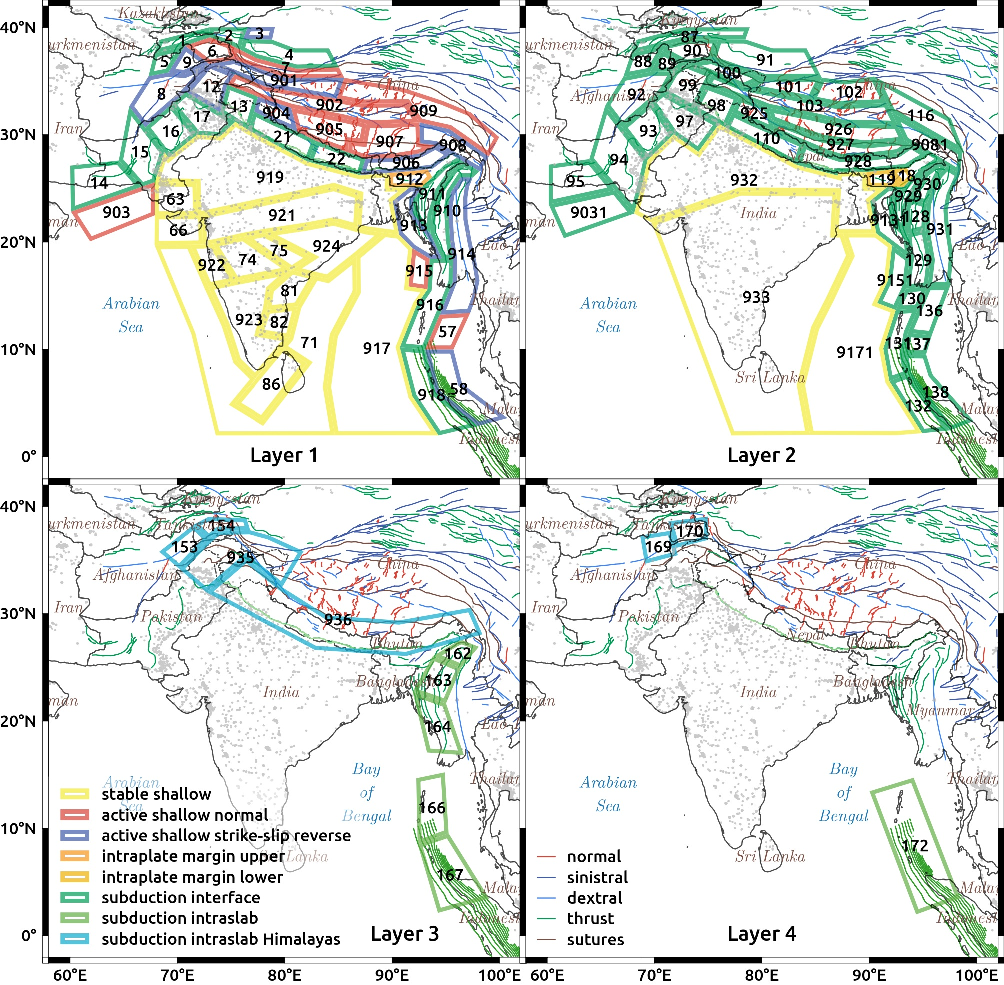
\includegraphics{India_Areal_Source_Model}
\end{adjustbox}
\caption[Areal source model]{Areal source model tectonic region assignments used in GMPE logic tree.
The areal source models is encoded in \texttt{\detokenize{areal_source_model.xml}}.
Zone identification numbers from \cite{nath2012probabilistic} are indicated.
Fault traces are from HimaTibetMap-1.0 \citep{styron2010database} except the Sumatran subduction fault which is from SLAB~1.0 \citep{hayes2012slab1}.
Fault data from the stable regions of India is lacking.
Urban areas, ``contiguous patches of built-up land greater than 1~km²'' \citep{schneider2009new}, are indicated in darker grey.}
\label{fig:ArealSourceModel}
\end{figure}

Potentially problematic tectonic region type assignments include:
\begin{itemize}
\item Zone 17 at the edge of the Pamir ranges is arguably ``stable shallow crust'' but was assigned ``subduction interface''.
\item Zone 906 in the Great Himalayas just north of the Shillong plateau was assigned ``active shallow crust strike-slip reverse'' even though the main trace of the Himalayan subduction fault runs through it, because the representative focal mechanism is strike-slip.
\item Zones 903 and 915-918 are predominantly oceanic crust but have been assigned ``active shallow crust'' or ``subduction interface'' according to the dominant focal mechanism and fault types.
For example zone 903 includes the Murray Ridge and so exhibits predominantly normal faulting as expected for a spreading ridge.
It is classified for the purpose of GMPE selection as ``active shallow crust normal'', but is likely in reality to produce ground motions distinct from an active continental crust.
\item Zones 71, 86 on layer 1 and zones 9031, 9081, 9131, 9151 and 9171 on layer 2 have have $a$ values of zero and so were assigned a ``no seismicity'' type and omitted from the areal source model.
\item Zones 169, 170 and 172 on layer 4 capture seismicity at 180-300 km depth, but only \cite{youngs1997strong} and \cite{kanno2006new} support depths below 180 km (see \autoref{table:GMPEs}).
\end{itemize}

Zones numbered as ``9xx'' in \cite{nath2012probabilistic} represent the amalgamation of several zones from \cite{thingbaijam2011seismogenic}.
In some cases this was done because of similarity of source mechanisms and statistics while in others it was necessary because the amount of seismicity in one of the zones was insufficient for FMD characterisation.
Furthermore, zones numbered ``9xx1'' in layer 2 have effectively had their seismicity transferred to the corresponding zones 9XX in layer 1.
For example zones 32 and 115 in \cite{thingbaijam2011seismogenic} become zones 908 and 9081 in \cite{nath2012probabilistic}, where zone 9081 has no seismicity.

Note that on layers 3 and 4 two distinct tectonic region types are defined for intraslab subduction \citep[p.
137]{nath2012probabilistic}.
Specifically, the ``Indo-Myanmar and Andaman-Sumatra subduction zones'' are assigned ``intraslab'' while the ``Himalayas and northwest India-Eurasia convergence'' are assigned ``intraslab Himalayas''.
Different GMPEs are applied in these regions, as described in \autoref{subsec:LogicTrees}, in particular the Japan and Cascadia adjustments of \cite{atkinson2003empirical} are applied, respectively.

Magnitude-scaling relations are used in PSHA to determine the actual rupture dimensions once a magnitude has been drawn from a frequency-magnitude distribution.
These were relatively straightforward to select once the tectonic region assignments were made, since ``\cite{wells1994new} for crustal events and those given by \cite{strasser2010scaling} for the subduction earthquakes'' \citep[p.~140]{nath2012probabilistic}.
It was inferred that for interface and intraslab regions \texttt{StrasserInterface} and \texttt{StrasserIntraslab} should be used, respectively.
The comment that ``the fault-rupture area estimated from the magnitude is constrained by a factor of 2'' \citep[p.~140]{nath2012probabilistic} was similarly interpreted as a width/depth aspect ratio of 2.

Since it is not explicitly stated in \cite{nath2012probabilistic} the seismogenic depth was assumed to be midway between the minimum and maximum for each layer.
Potential refinements to this setup are discussed in \autoref{app:SourceModelImprovements}.

The supplementary information required to generate the fully specified areal source model from the electronic supplement files \texttt{polygonlay\%d.txt} and \texttt{seismicitylay\%d.txt} files in the is contained in \texttt{auxiliary data.csv}.

\subsubsection{Smoothed-gridded}
\label{subsubsec:Smoothed}

Smoothed-gridded seismicity models aim to replicate geographic variations of activity rates in a catalogue-driven way.
Typically a smoothing kernel is used which enforces a correlation distance and limits the resolution.

Some details of the smoothing are contained in the unpublished \cite{thingbaijam2011seismogenic}: a Gaussian kernel was used, following the methodology of \cite{frankel1995mapping} with correlation distances of 65 and 85~km for $m_{min}$ of 4.5 and 5.5 respectively.

After some discussion with K.
Thingbaijam it was decided that although the models are described as ``spatially varying annual activity rates'' \cite[p.~140]{nath2012probabilistic} the electronic supplement actually contains spatially smoothed total seismicity, i.e. number of events (per cell).
In order to convert this information to activity rates, i.e. number of events per year (per cell), it was necessary to obtain the duration of each sub-catalogue.
Fortunately this missing ingredient is summarized in \cite[Table 1]{thingbaijam2011seismogenic} and reproduced in \autoref{table:Completeness}.

Given the total seismicity $N$ and the length in years of the relevant catalogue $T$ (see \autoref{table:Completeness}) the annual rate $\nu$ for a given model is obtained using:
\begin{equation} \label{eq:SeismicityToActivity} 
\nu = N/T 
\end{equation}

In OpenQuake each point in the smoothed seismicity model is treated as a point source with a specified frequency-magnitude distribution: at a minimum $a$, $b$ and $m_{max}$ must be spedified.
\cite{nath2012probabilistic} indicate that ``$b$-value and $m_{max}$ remain fixed within the source zone''.
Thus in the present study for the smoothed seismicity model the parameters $b$ and $m_{max}$ of the truncated Gutenberg-Richter magnitude-frequency distributions are inferred from the areal source model zonation.
For points inside zones with non-zero $a$ values in the areal source model this is trivial; for points outside these zones the zone with the shortest perpendicular distance to the point was chosen.

A gridded point source model also requires specification of  tectonic region type and source mechanism for the selection and implementation of GMPEs, as well as the uncertainty in the FMDs.
Thus the same procedure was used to assign tectonic subregion, rake, dip, strike, magnitude scaling relations, $\sigma_b$ and $\sigma_{m_{max}}$.

The truncated Gutenberg-Richter magnitude-frequency distribution in OpenQuake implements

$$ \lambda(M \geq m) = 10^{a - b m} = e^{\alpha - \beta m} $$

Ignoring events below some threshold $m_{min}$, the annual rate becomes

$$ \lambda(M \geq m_{min}) = e^{\alpha - \beta m_{min}} e^{-\beta (m - m_{min})} = \nu e^{-\beta (m - m_{min})} $$

Thus to compute the $a$ value for a point source from the activity rate $\nu$ for a given magnitude threshold, we take into account the $b$ value for the zone as follows:

$$a = \log_{10}(\nu) + b m_{min} $$

Similarly to compute the activity rate for an areal source we can use

\begin{equation} \label{eq:ArealActivity} 
\nu = 10^a - 10^{b m_{min}}
\end{equation}

In order to verify that the smoothed and areal models are approximately equivalent to each other and the catalogue, annual activity rates were computed for each.
Areal activity rates were computed using \eqref{eq:ArealActivity}.
Smoothed model activity rates were computed by summing the seismicity for all points and then applying \eqref{eq:SeismicityToActivity}.
Catalogue activity rates were computed by querying the catalogue of \cite{nath2010earthquake} with appropriate minimum magnitudes and within the bounds of the areal source model.
Note also that events are only counted if the epicentre is within one of the zones of the areal model.
This was done on a layer-by-layer basis as well as over the whole model.

The results are tabulated in \autoref{table:Rates}.
Both the areal and smoothed models tend to overestimate the seismicity in the catalogue.
Discrepancies between the areal model and the catalogue are likely an artefact of taking the total seismicity for a given zone, computing a frequency-magnitude distribution, and applying that FMD uniformly over the zone.
Discrepancies between the smoothed model and the catalogue cannot be explained by the smearing effect of the smoothing kernel, because this should result in smoothed seismicity rates lower than the catalogue rates when computed over the same area, whereas we observe smoothed seismicity rates which are higher.
Improvements to the smoothed seismicity model are proposed in \autoref{app:SourceModelImprovements}.

\begin{table}
\caption[Comparison of annual seismicity rates]{Comparison of annual seismicity rates for areal model, smoothed-gridded seismicity model and catalogue.
In each case the value shown is the average or expected number of events per year $\nu$ above the given minimum magnitude.
Catalogue events and smoothed-gridded point sources are only counted if the epicentre is within one of the zones of the areal model.}
\label{table:Rates}
\centering
\begin{tabular}{ccccccc}
\toprule
$m_{min}$ & \multicolumn{3}{c}{4.5} & \multicolumn{3}{c}{5.5} \\
source &  areal & smoothed & catalogue & areal & smoothed & catalogue \\
\midrule
layer   &      &        &         &       &          &           \\
1       &   80 &    130 &      54 &   8.4 &      4.1 &       3.1 \\
2       &   68 &    174 &      78 &  10.4 &      3.6 &       3.8 \\
3       &   36 &     89 &      40 &   2.9 &      1.7 &       1.6 \\
4       &   12 &     43 &      10 &   1.6 &      1.2 &       1.2 \\
total   &  194 &    435 &     182 &  23.3 &     10.6 &       9.7 \\
\bottomrule
\end{tabular}
\end{table}

\begin{figure}[!htb]
\begin{adjustbox}{center}
\includegraphics{India_Smoothed_Source_Model}
\end{adjustbox}
\caption[Smoothed seismicity point source model]{Tectonic region assignments and activity rates for smoothed seismicity point source model.
The smoothed seismicity source models are encoded in \texttt{\detokenize{smoothed_source_model_mmin4.5.xml}} and \texttt{\detokenize{smoothed_source_model_mmin5.5.xml}}}
\label{fig:SmoothedSourceModel}
\end{figure}

Other issues of note:
\begin{itemize}
\item Zones 9031, 9081, 9131, 9151 and 9171 on layer 2 have $m_{max}$ values values of zero.
These zones all the the smoothed seismicity points in or nearest to these zones on layer 2 were assigned the $m_{max}$ values from the corresponding zones on layer 1, namely zones 903, 908, 913, 915 and 917.
\item Given that the Japan/Cascadia regional adjustments are used for intraslab subduction, it is not clear why they are not also applicable for interface subduction.
\item Although the hazard maps in the electronic supplement are at 0.2° and the paper says the smoothed-gridded models are also at 0.2° they are in fact at 0.1°.
\autoref{fig:SmoothedSourceModel} shows the model at just 0.2° for convenience.
\end{itemize}

\subsection{Ground-motion prediction}
\label{subsec:GroundMotion}

In order to evaluate seismic hazard across the Indian subcontinent it is necessary to consider 

The great Assam earthquake of 1897 destroyed buildings within several hundred km.
The two main fault structures involved are capable of M > 8 plateau-building events with a recurrence interval of 3-8 kyr each \citep{bilham2001plateau}.

\cite{nath2012ground} notes stress drop apparently increasing with depth and models $\kappa$ using a database of recent well-recorded micro-earthquakes, and uses this information to develop stochastic models for events in the upper and lower crust.
The simulations are of vertical motion at a hard-rock site and no site corrections are attempted.

\cite{sharma2009ground} points out that the decay rate of PGA for shallow India-Bangladesh and deep India-Burma border events have different distance scaling.
The former leads to the necessity of a GMPE specific to the Shillong plateau \cite{nath2012ground} while the latter means interface subduction events need to be treated differently.

Issues encountered while implementing GMPE logic tree:
\begin{itemize}
\item layer~4 depth range of 180-300~km is significantly deeper than deepest events used in regression for ATBO03 (100 km), LILE08 (161 km), ZHAO06 (120 km) and GUPT10 (148 km) are specified for.
YCSH97 only included events to 229 km.
KANN06 is specified to 200 km depth, but is only used for interface events (layer~2).
\item Assumed “and Andaman-Sumatra subduction” missing from Figure 3.
\item Why is Youngs (1997) not used in the subduction interfaces?
\item \cite{nath2012probabilistic} doesn't seem to me to follow the recommendations of \cite{nath2011peak} as far as having two subduction intra-slab sub-regions: the former uses Indo-Myanmar and Himalayas while the latter recommends Indo-Myanmar and Hindukush.
\cite{nath2012probabilistic} is followed strictly for for phase 1.
\item Assignment of source mechanism (normal or not, matters in shallowest layer only) is tricky.
 Dip cannot be used to distinguish normal and reverse subduction because the subduction interface angle is not known.
different GMPEs use different rake thresholds; a threshold of 30\degree\space was chosen, consistent with \cite{boore2008ground, campbell2008nga} but not \cite{zhao2006attenuation}.
\end{itemize}

Issued encountered while implementing GMPEs:

\cite{sharma2009ground}
\begin{itemize}
\item lacks a $M^2$ term \cite{cotton2006criteria}
\item does not define PGA (inferred from 0.04 Hz)
\end{itemize}

\cite{raghukanth2007estimation}
\begin{itemize}
\item typographical errors in coefficient tables: grossest error fixed, 3 other errors causing approximately 10\% error not fixed
\item actually defines 4 different models: must assume that for all of peninsular India was used by \cite{nath2012probabilistic}, not one of those for sub-regions.
\end{itemize}

\begin{table}
\caption[Ground motion prediction equations]{Ground motion prediction equations used in this study.
Citations can be inferred from OpenQuake class names.
``N'' indicates that models were newly implemented in OpenQuake for the current study.
``S'' indicates that the model has since been superseded by an equivalent model from the same authors.
Among the databases used, ``ENA'' stands for eastern North America, and ``NGA'' stands for next generation attenuation.
The tectonic region ``Type'' uses the following abbreviations:
    ``active'' shallow crust,
    ``intraplate'' margin,
    ``stable'' continental crust,
    ``interface'' subduction and
    ``intraslab'' subduction.
$N_E$ and $N_R$ are the number of earthquakes and records in the database, respectively.
$H$, $M$ and $R$ are the ranges of depth, magnitude and distance over which the GMPE is considered by the authors to be valid.}
\label{table:GMPEs}
\centering
\begin{adjustbox}{width=1.2\textwidth,center=\textwidth} ..
\begin{tabular}{lcccccccccccc}
\toprule
OpenQuake class & N & S & Database & Type & $N_E$ & $N_R$ & \multicolumn{2}{c}{$H$ [km]} & \multicolumn{2}{c}{$M$} &  \multicolumn{2}{c}{$R$ [km]} \\
\midrule
\texttt{AkkarBommer2010}                &             &  \checkmark & \begin{tabular}{c}Europe \& \\ Middle East\end{tabular} &   active   &               131 &    532 &             &             &         5.0 &          7.6 &              0 &          100 \\
\texttt{BooreAtkinson2008}              &             &  \checkmark &               NGA-West &   active   &                58 &   1574 &             &             &         5.0 &          8.0 &              0 &          200 \\
\texttt{CampbellBozorgnia2008}          &             &  \checkmark &               NGA-West &   active   &                72 &    942 &             &             &         4.0 &          8.0 &              0 &          200 \\
\texttt{Kanno2006Shallow}               &  \checkmark &             &                  Japan &   active   &                83 &   3769 &           0 &          30 &         5.5 &          8.2 &                &          450 \\
\texttt{SharmaEtAl2009}                 &  \checkmark &             & \begin{tabular}{c}Himalayas \&\\Zagros\end{tabular} &   active   &                16 &    201 &             &             &         5.0 &          7.0 &                &          100 \\
\texttt{NathEtAl2012Upper}              &  \checkmark &             & Shillong               & intraplate & \multicolumn{2}{c}{simulation} &       0 &          25 &         4.8 &          7.6 &             10 &          100 \\
\texttt{NathEtAl2012Lower}              &  \checkmark &             & Shillong               & intraplate & \multicolumn{2}{c}{simulation} &      25 &          40 &         4.8 &          8.1 &             10 &          100 \\
\texttt{AtkinsonBoore2006}              &             &             & ENA                    &   stable   &                10 &  34800 &           2 &          30 &         5.0 &          8.3 &                &         1000 \\
\texttt{Campbell2003}                   &             &             & ENA                    &   stable   & \multicolumn{2}{c}{hybrid} &   &             &         5.0 &          8.2 &              0 &         1000 \\
\texttt{RaghukanthIyengar2007}          &  \checkmark &             &\begin{tabular}{c}Peninsular\\India\end{tabular} &   stable   & \multicolumn{2}{c}{simulation} &       5 &          15 &         4.0 &          8.0 &                &          300 \\
\texttt{ToroEtAl2002}                   &             &             & ENA                    &   stable   & \multicolumn{2}{c}{simulation} &             &             &         5.0 &          8.0 &                &         1000 \\
\texttt{Kanno2006Deep}                  &  \checkmark &             &                  Japan & subduction &               111 &   8150 &          30 &         200 &         5.5 &          8.2 &                &          450 \\
\texttt{AtkinsonBoore2003SInter}        &             &             &                 global &  interface &                80 &   1155 &          20 &          50 &         5.0 &          8.3 &             10 &          550 \\
\texttt{ZhaoEtAl2006SInter}             &             &  \checkmark &                  Japan &  interface &               269 &   1520 &          25 &          50 &         5.0 &          8.3 &                &          300 \\
\texttt{AtkinsonMacias2009}             &             &             &               Cascadia &  interface & \multicolumn{2}{c}{simulation} &         &             &         7.5 &          9.0 &                &          400 \\
\texttt{AtkinsonBoore2003SSlabJapan}    &  \checkmark &             &                 global &  intraslab &                80 &   1155 &          50 &         100 &         5.0 &          8.3 &             30 &          550 \\
\texttt{AtkinsonBoore2003SSlabCascadia} &  \checkmark &             &                 global &  intraslab &                80 &   1155 &          50 &         100 &         5.0 &          8.3 &             30 &          550 \\
\texttt{LinLee2008SSlab}                &             &             & NE Taiwan               &  intraslab &                54 &   4823 &          39 &         161 &         4.1 &          6.7 &             40 &          600 \\
\texttt{Gupta2010SSlab}                 &  \checkmark &             & \begin{tabular}{c}Indo-\\Myanmar\\Arc\end{tabular} &  intraslab &                 3 &     56 &          91 &         148 &         6.3 &          7.2 &                &          375 \\
\texttt{YoungsEtAl1997SSlab}            &             &             &                 global &  intraslab &               164 &    480 &          50 &         229 &         5.0 &          7.8 &             10 &          500 \\
\texttt{ZhaoEtAl2006SSlab}              &             &  \checkmark &                  Japan &  intraslab &               269 &   1725 &          50 &         120 &         5.0 &          8.3 &                &          300 \\
\bottomrule
\end{tabular}
\end{adjustbox}
\end{table}

\cite{kanno2006new} -> \cite{douglas2003earthquake}

\subsection{Logic Trees}
\label{subsec:LogicTrees}

\subsubsection{Ground-Motion Prediction}
\label{subsubsec:GmpeTree}

The GMPE logic tree implemented in \cite{nath2012probabilistic} is shown in \autoref{fig:GmpeTreeNath}.
Since some of these GMPEs are new to OpenQuake (see \autoref{table:GMPEs}) a comparison was done between that model and that obtained with only the standard GMPEs.
For this purpose a "simplified" GMPE logic tree was constructed which simply omitted the newly-implemented GMPEs and retained equal weighting for the rest.

\begin{figure}[!htb]
\begin{adjustbox}{center}
\includegraphics{gmpe_logic_tree_omit_new.pdf}
\end{adjustbox}
\caption[Simplified GMPE logic tree]{Simplified GMPE logic tree employing only established OpenQuake models, as encoded in \texttt{\detokenize{gmpe_logic_tree_omit_new.xml}}.
Middle column selects tectonic region types as defined in \autoref{fig:ArealSourceModel}.
OpenQuake model class names and assigned weights are given on the right side.
New and established classes are summarized in \autoref{table:GMPEs}}
\label{fig:GmpeTreeSimplified}
\end{figure}

\begin{figure}
\begin{adjustbox}{center}
\includegraphics{gmpe_logic_tree.pdf}
\end{adjustbox}
\caption[Original GMPE logic tree]{GMPE logic tree of \cite{nath2012probabilistic}, as encoded in \texttt{\detokenize{gmpe_logic_tree.xml}}.
See \autoref{fig:GmpeTreeSimplified} for complete description}
\label{fig:GmpeTreeNath}
\end{figure}

Moving forward an obvious modification is to replace superseded NGA models with their more up-to-date versions.

[It may also be desirable to rationalize the weighting of the GMPEs or include entirely new ones, such as the new BC Hydro subduction model \citep{abrahamson2012bc}.
The discussion continues below and is incomplete.]

\cite{anbazhagan2015selection} seem to be proposing different weights for different regions based on single events in those regions.
An extreme example is to define different weights for Anjar, 1956 and Bhuj , 2001 earthquakes even though the epicentres and depths were very close together.
In contrast \cite{nath2011peak} compute LLH for 7 regions (using 38 events total) and state that, ``individual events do not have significant number of observations to support a viable ranking basis.''

\cite{anbazhagan2015selection} seem to misuse the concept of data support index (DSI) \citep{delavaud2012toward} by setting weights to zero when the DSI is negative.
The threshold is arbitrary and is chosen without discussion.
As \cite{delavaud2012toward} point out ``more important
than the sign of the DSI is the difference of DSI between
two models.''

Both \cite{anbazhagan2015selection} and \cite{nath2011peak} rely on estimating ground motions from macroseismic intensity.
I'm sure it is a matter of low seismicity and lack of instrumentation, but I'm still surprised.
I would expect the catalogue for peninsular India to be complete for 20 years to magnitude 5 so that one could thus get 10 well-recorded events, at least.
There is significant additional (aleatory and epistemic) variability in mapping EMS to PGA which must obscure the true performance of the GMPEs.
 Perhaps this is part of why  \cite{anbazhagan2015selection} and \cite{nath2011peak} arrive at such different LLH scores and rankings for the same events \cite[][Table 5]{anbazhagan2015selection}.
It would be interesting to compare the results of LLHs computed using EMS inferred from digitized intensity maps to those computed using instrumental PGA for at least a few events since 1990.
\cite{nath2011peak} take a step towards this by looking at the scatter in their mapping of PGA to EMS but it's not quite the same.

Many authors \citep{scherbaum2009model, nath2011peak, delavaud2012toward, anbazhagan2015selection} seem unduly interested in "ranking", i.e. constructing an ordered list of GMPEs.
This is not a horse race.
\cite{scherbaum2009model} suggests a way to turn an LLH score into a logic-tree weight and the formula does not require ranking.
Furthermore, in constructing a logic tree one must include factors outside the performance-based scoring, for example an assessment of whether the set is ``mutually exclusive and collectively exhaustive'' \citep{bommer2008use}.
For me the question of ranking is just "noise" which obscures more important questions.

The mutual exclusivity requirement means, to me, that models should be omitted which are redundant in the sense of being too similar to other models in terms of the methodology of their construction, especially if that means they make similar predictions and have similar limitations as a result.
For example the exclusion of models which have been superseded \citep{cotton2006criteria} can be seen as an application of the requirement that models be mutually exclusive.
Another example would be, for a GMPE logic tree intended for the Indian subcontinent, to omit a model such as \cite{hwang1997attenuation} in favour of \cite{atkinson2006earthquake} since both are based on stochastic simulation in Eastern North America.

The collective exhaustiveness requirement means, is trickier.
It is this requirement which pushes hazard modellers to seek out and evaluate more and complementary types of models.
Thus models with broad data support from other regions complement models with poor data support from the target region.
Stochastic models supplement data-driven models.
Models with different functional forms, distance or magnitude ranges can complement each other.

The process of developing a logic tree to assess epistemic uncertainty is thus a dialectical one.
Mutual exclusivity and collective exhaustiveness comprise opposing forces which must be exerted alternately and in tandem.

[Now apply these principles to move forward from \cite{nath2012probabilistic}!] 

\subsubsection{Source Models}
\label{subsubsec:SourceTree}

The source model logic tree is shown in symbolic form in \autoref{fig:SourceTreeSymbolic}.

\begin{figure}[!htb]
\begin{adjustbox}{center}
\includegraphics{source_model_logic_tree_symbolic.pdf}
\end{adjustbox}
\caption[Symbolic source model logic tree]{Symbolic source model logic tree of \cite{nath2012probabilistic}.}
\label{fig:SourceTreeSymbolic}
\end{figure}

\cite{nath2012probabilistic} accounts for the epistemic uncertainty in seismicity model parameters by estimating the standard deviations of $b$ and $m_{max}$ in each source zone and assigning weights to ±1 standard deviation for each source.
This results in a source model logic tree too large to represent on a page; just a portion of it is shown in \autoref{fig:SourceTreePartial}.

\begin{figure}
\begin{adjustbox}{center}
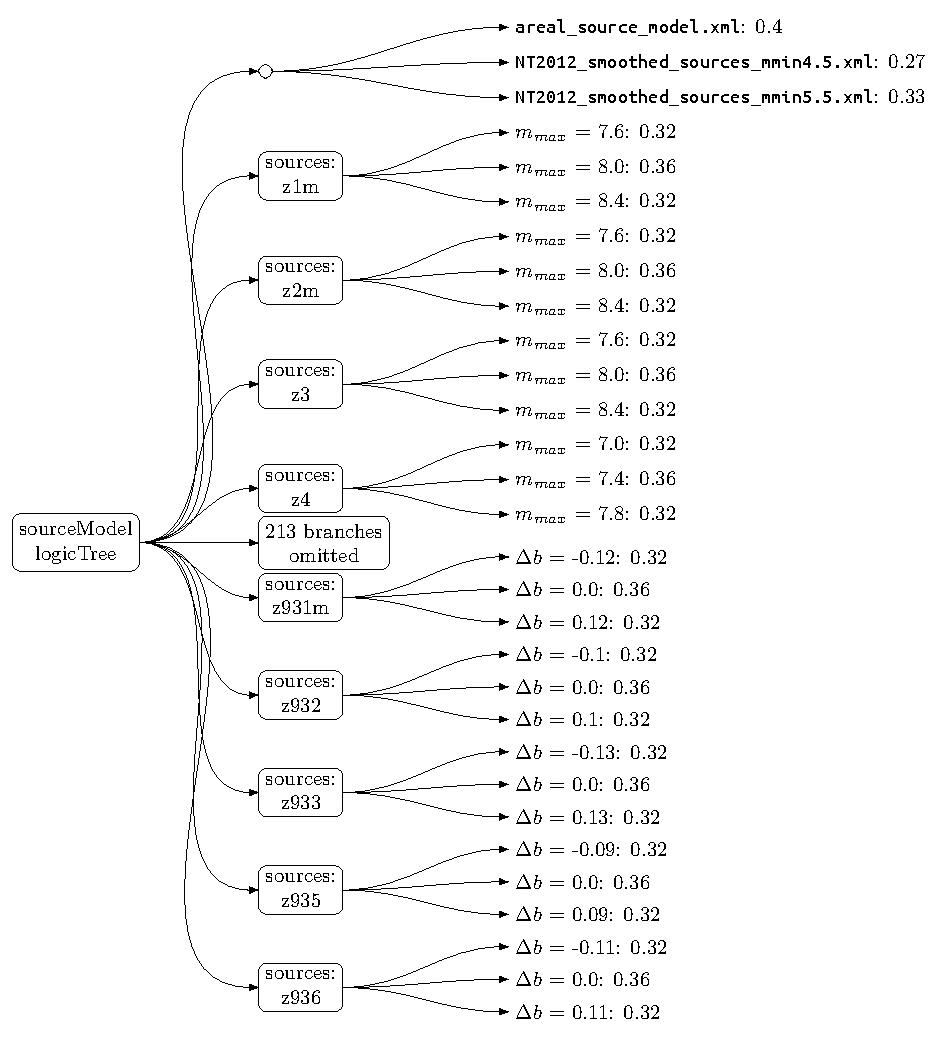
\includegraphics{source_model_logic_tree.pdf}
\end{adjustbox}
\caption[Partial source model logic tree]{Partial source model logic tree of \cite{nath2012probabilistic}.
The full model is encoded in \texttt{\detokenize{source_model_logic_tree.xml}}}
\label{fig:SourceTreePartial}
\end{figure}

Note that although Figure 4 of \cite{nath2012probabilistic} shows the activity rate $\nu$ (and by implication $a$) varying with $b$, no estimates of the standard deviation of $a$ or $nu$.
The  in OpenQuake happens to recalculate $a$ as $b$ After modifying $b$ using the uncertainty type \texttt{bGRRelative} the $a$ value is automatically recalculated to maintain constant total moment rate.
It has been assumed that this is the behaviour which \cite{nath2012probabilistic} implemented.

The fact that \autoref{fig:SourceTreePartial} has to be truncated is not simply a lack of page space.
Despite the common rendering of them in parallel, full enumeration actually takes place in series, so rather than just 3$\times$223 branches there are in fact $3^{223} \approx 10^106$, or just over a googol of branches.
Not only was full-enumeration out of the question, even partial enumeration was problematic on the current version of OpenQuake code.

It is unlikely that \cite{nath2012probabilistic} performed full-enumeration.
Some practitioners 

\section{Hazard results}
\label{sec:Results}

\subsection{Verification}
\label{subsec:Verification}

Validation of PSHA results would require comparison against observed hazard, and would require a much larger dataset than is currently available.
In this work we are merely verifying that the current model gives result close to those of \cite{nath2012probabilistic}.

\subsection{Sensitivity}
\label{subsec:Sensitivity}

\subsection{Discussion}
\label{subsec:Discussion}

\section{Conclusions}
\label{sec:Conclusions}

\section*{Acknowledgement}
Thanks to Kiran Thingbaijam for clarifications and engaging discussion.
Thanks to Amanda for your support.

\cleardoublepage
\phantomsection
\addcontentsline{toc}{section}{Bibliography}
\bibliographystyle{apalike}
\bibliography{/home/nick/Desktop/Library/PSHA.bib,/home/nick/Desktop/Library/india-hazard.bib}

\begin{appendices}

\section{Alternative GMPEs}
\label{app:AlternativeGmpes}

\section{Catalogue Evaluation}
\label{app:Catalogue}

\section{Potential Source Modelling Improvements}
\label{app:SourceModelImprovements}

\begin{figure}[htb]
\begin{adjustbox}{center}
\includegraphics{Depth_histogram_(mainshocks)}
\end{adjustbox}
\caption[Depth histogram for mainshocks]{Depth histogram for mainshocks over magnitude 5.5.
Mainshock identification is that of \cite{nath2010earthquake}.
Seismogenic layer boundaries and hypocentral depths used in the current implementation are indicated as dashed and dash-dotted lines respectively.}
\label{fig:DepthHistogram}
\end{figure}

\begin{figure}[!htb]
\begin{adjustbox}{center}
\includegraphics{Depth_vs_distance_(mainshocks)}
\end{adjustbox}
\caption[Depth vs.
distance for mainshocks in regions with deep events]{Depth vs.
distance for mainshocks in regions with deep events.
Subregions are indicated on each map; top left is the Hindu-Kush and Pamir ranges in the northwest of India viewed from the east, top right is the Andoman-Sumatran subduction zone viewed from the south while bottom left and right are beneath the Indoburman range and viewed from the east and south respectively.
Sub-catalogues were selected for events over magnitude 5.5 within a rectangular box of latitude and longitude as indicated on each individual plot.
 Horizontal and vertical axes are plotted at different scales.}
\label{fig:DepthVsDistance}
\end{figure}

\begin{itemize}
\item Base hypocentral depths on actual seismogenic depth distribution as shown in \autoref{fig:DepthHistogram}.
Placing the hypocentral depth at the modes of the overall catalogue would be a minor improvement.
Better still would be to capture the mode or to construct an approximate distribution for each areal zone.
\item Model the main Himalayan thrust as a simple fault.
In particular \cite{berryman2014himalayan} breaks the fault into three segments and provides necessary details such as dip and depth limits.
No variation of dip with depth is given, which is perhaps unrealistic, but at least the result is simpler to model.
Not all of the slip is being taken up on the frontal thrust; there are second and third folds which take up significant amount of slip, but the first is the most important from the standpoint of risk.
\item Model the Oldham and Dauki faults under the Shillong plateau as simple faults \citep{Bilham2001}.
\end{itemize}

\section{Summary of Electronic Data}
\label{app:Jobs}

This is an appendix because if you're reading this then you should already have the zip file with all of this data.

\texttt{auxiliary data.csv} 

\lstinputlisting[language=Ini,caption=\lstname]{phase1-job.ini}

\end{appendices}

\end{document}